\chapter{Propuesta}\label{approach}

\section{Consideraciones Iniciales}
En la presente tesis se propone un enfoque innovador para la detección de fases sísmicas utilizando modelos basados en Transformers, específicamente EQTransformer. Este modelo ha demostrado ser efectivo en la clasificación de eventos sísmicos y se adapta bien a las limitaciones de recursos computacionales, lo que lo hace adecuado para aplicaciones en tiempo real y sistemas de alerta temprana.

El objetivo principal es evaluar el rendimiento de EQTransformer en la detección de ondas P y S, comparándolo con otros modelos basados en Transformers y enfoques tradicionales. Se busca determinar la viabilidad de estos modelos para su implementación en sistemas de monitoreo sísmico, especialmente en entornos con recursos limitados. Y ademas proponer mejoras en la arquitectura y el entrenamiento del modelo para optimizar su rendimiento. Para lograr esto, se utilizarán conjuntos de datos de sismogramas etiquetados, y se realizarán experimentos para medir la precisión, la recuperación y la puntuación F1 de los modelos en la detección de fases sísmicas. La principal contribución de esta tesis es demostrar que los modelos basados en Transformers, como EQTransformer, pueden superar a los enfoques tradicionales en la detección de ondas P y S, ofreciendo una alternativa robusta y eficiente para el análisis sísmico.

\section{Estructura del Pipeline}

El pipeline propuesto para la detección de fases sísmicas P y S se compone de varias etapas clave, que incluyen la preparación de datos, el entrenamiento del modelo y la evaluación de resultados. A continuación, se describen las principales etapas del pipeline:

\begin{figure}
\centering
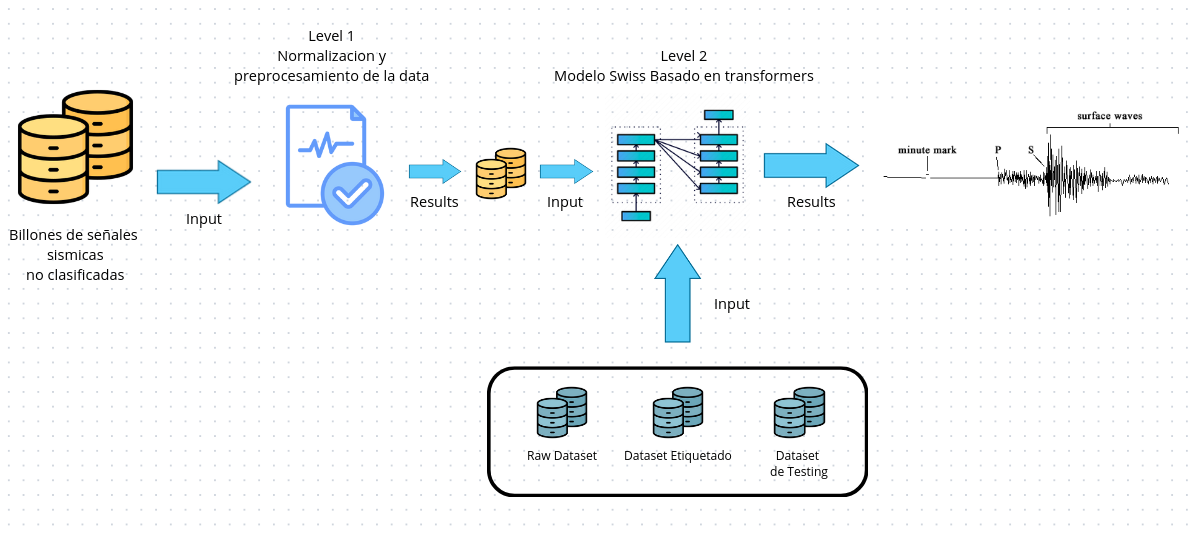
\includegraphics[width=0.8\textwidth]{figures/PIPELINE.png}
\caption{Estructura del Pipeline Propuesto}
\label{fig:pipeline}
\end{figure}

La Figura \ref{fig:pipeline} ilustra el flujo de trabajo del pipeline, que comienza con la preparación de los datos. Se explica mas a detalle en la sección \ref{sec:Dataset}.

La preparacion de la data consiste en la recolección de sismogramas etiquetados con las fases P y S, que son fundamentales para el entrenamiento del modelo. Estos datos se procesan para extraer características relevantes que serán utilizadas por el modelo.

El siguiente paso es el entrenamiento del modelo, donde se utiliza el dataset preparado para ajustar los parámetros del modelo EQTransformer. Durante esta etapa, se optimizan los pesos del modelo utilizando un optimizador Adam con una tasa de aprendizaje adaptativa, lo que permite una convergencia eficiente y efectiva.

El modelo presentado tiene la siguiente estructura:

\begin{figure}
\centering
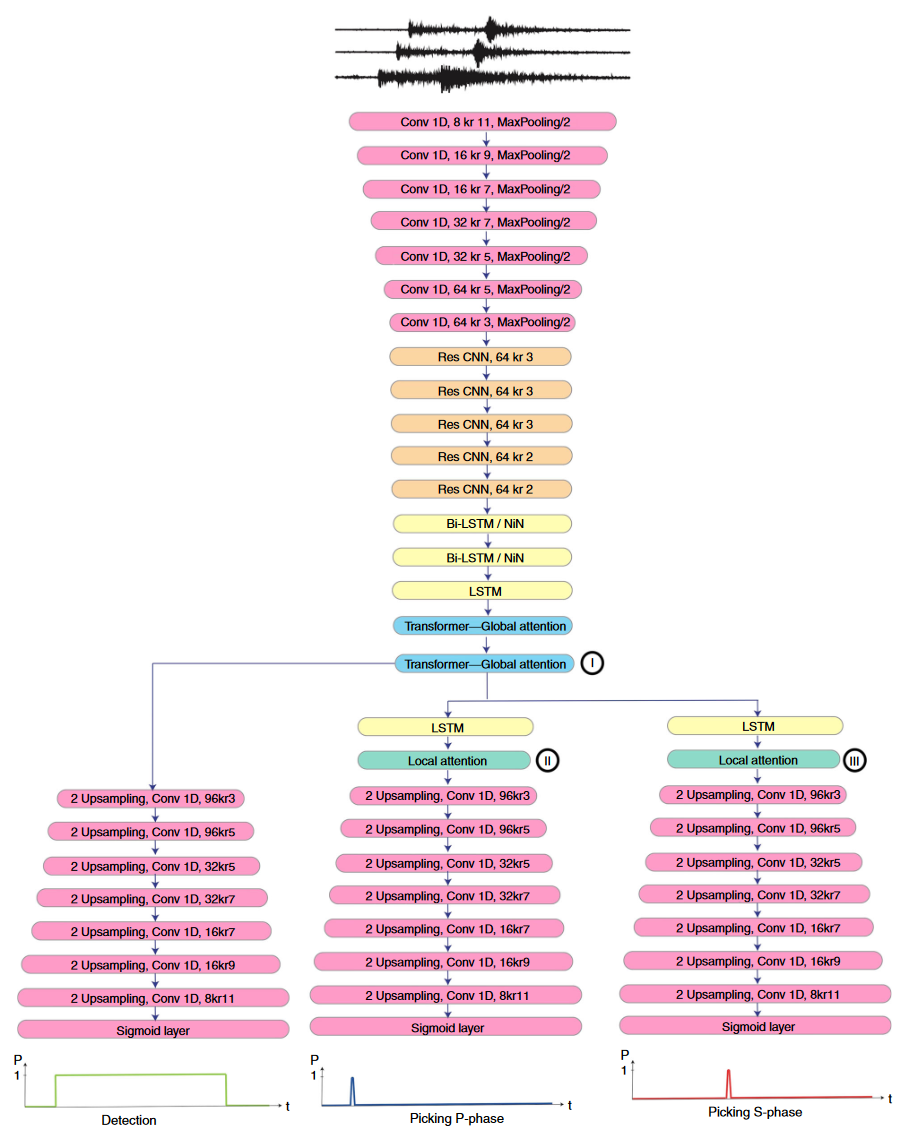
\includegraphics[width=0.8\textwidth]{figures/transformer.png}
\caption{Estructura del Modelo EQTransformer}
\label{fig:eqtransformer}
\end{figure}

La Figura \ref{fig:eqtransformer} muestra la arquitectura del modelo EQTransformer, que combina un módulo de Atención por Coordenadas con un mecanismo de atención de Transformers. Esta estructura permite una mejor captura de las características relevantes en los sismogramas, mejorando así la precisión y recuperación en la detección de fases sísmicas.



La evaluación de resultados implica medir el rendimiento del modelo en términos de precisión, recuperación y puntuación F1. Estas métricas son esenciales para determinar la efectividad del modelo en la detección de fases sísmicas P y S.

\section{Esquema de la Propuesta}

La innovación del marco propuesto en esta tesis radica en la integración del módulo de Atención por Coordenadas (Coordinate Attention) con el mecanismo de atención de Transformers, y la implementación de una estructura de modelo híbrido que combina Transformers y redes convolucionales a través de un módulo de concatenación, como se muestra en la Figura 4. 

A través de la función del módulo de Atención por Coordenadas (Ecuaciones \ref{eq:conv1d} y \ref{eq:sigmoid}), las características de entrada se transforman en características mejoradas $Z$, haciendo que las características clave en los datos originales sean más prominentes. El objetivo es resaltar la información crucial dentro de la matriz de características de entrada $X$. 

En arquitecturas de aprendizaje profundo, las conexiones residuales son una técnica ampliamente utilizada que permite la transferencia directa de información entre diferentes capas. Esta técnica es particularmente importante para la construcción de redes profundas, ya que ayuda a mitigar los problemas de gradientes que desaparecen o explotan, permitiendo así el entrenamiento de redes más profundas.

\begin{equation}
Y = \text{Conv1d}(X; \text{kernel size} = 1, \text{stride} = 1)
\label{eq:conv1d}
\end{equation}

\begin{equation}
Z = \sigma(Y)
\label{eq:sigmoid}
\end{equation}

Donde $\sigma(Y)$ representa la función Sigmoide. La característica mejorada $Z$ se divide posteriormente en tres flujos de procesamiento independientes. Un flujo procesa a través de una red neuronal convolucional unidimensional con parámetros $\text{kernel size} = 1$ y $\text{stride} = 1$ para calcular el valor de consulta $Q$ para el Transformer, como se describe en la Ecuación \ref{eq:query}.

\begin{equation}
Q = \text{Conv1d}(Z; \text{kernel size} = 1, \text{stride} = 1)
\label{eq:query}
\end{equation}

En otro flujo de procesamiento, los datos se someten a un submuestreo y se reducen dimensionalmente a través de las ecuaciones \ref{eq:downsampling}, \ref{eq:key}, y \ref{eq:value} para derivar las claves $K$ y los valores $V$ para el mecanismo de atención, un proceso destinado a reducir la complejidad computacional.

\begin{equation}
Z' = \text{DownSampling}(Z)
\label{eq:downsampling}
\end{equation}

\begin{equation}
K = \text{Conv1d}(Z'; \text{kernel size} = 1, \text{stride} = 1)
\label{eq:key}
\end{equation}

\begin{equation}
V = \text{Conv1d}(Z'; \text{kernel size} = 1, \text{stride} = 1)
\label{eq:value}
\end{equation}


\section{Arquitectura del Modelo}

El modelo propuesto tiene una estructura de red neuronal multitarea que consta de un codificador (\textit{encoder}) muy profundo y tres decodificadores (\textit{decoders}) separados. Cada componente está diseñado para abordar diferentes aspectos de la detección de señales sísmicas, como se detalla a continuación:

\subsection{Codificador (Encoder)}

El codificador es responsable de procesar las señales sísmicas en el dominio temporal y generar representaciones de alto nivel que capturen información contextual y dependencias temporales. Este módulo incluye las siguientes características clave:

\begin{itemize}
    \item \textbf{Sección de Submuestreo:} Para reducir la complejidad computacional, el codificador comienza con una sección de submuestreo compuesta por capas convolucionales y de \textit{max-pooling}. Estas capas disminuyen la longitud de la secuencia de entrada, permitiendo que el modelo maneje eficientemente señales largas.
    \item \textbf{Bloques Residuales de Convolución y LSTM:} Las características submuestreadas se transforman en representaciones de alto nivel mediante una serie de bloques residuales que combinan convoluciones unidimensionales (1D) y LSTM bidireccionales. Las conexiones residuales permiten entrenar redes profundas al mitigar problemas de gradientes que desaparecen o explotan.
    \item \textbf{Atención Global:} Al final del codificador, se incluye una sección de atención global que dirige el enfoque de la red hacia las partes de la señal asociadas con eventos sísmicos. Este mecanismo mejora la capacidad del modelo para identificar características relevantes en señales ruidosas.
\end{itemize}

\subsection{Decodificadores (Decoders)}

El modelo cuenta con tres decodificadores separados, cada uno diseñado para mapear las representaciones de alto nivel generadas por el codificador a secuencias de probabilidades asociadas con diferentes tareas:

\begin{itemize}
    \item \textbf{Decodificador de Detección:} Este decodificador utiliza directamente las características de alto nivel para generar una secuencia de probabilidades que indica la existencia de una señal sísmica en cada punto temporal.
    \item \textbf{Decodificadores de Fases P y S:} Los otros dos decodificadores están dedicados a la detección de las fases P y S, respectivamente. Cada uno comienza con una unidad de atención local que dirige el enfoque del modelo hacia características específicas dentro de la forma de onda sísmica asociadas con las fases individuales. Posteriormente, las características se procesan mediante bloques LSTM y capas completamente conectadas para generar las probabilidades correspondientes.
\end{itemize}

\subsection{Detalles de Implementación}

\begin{itemize}
    \item \textbf{Capas de Atención y Residuales:} Las capas de atención y las conexiones residuales dentro de cada bloque permiten al modelo mantener un equilibrio entre profundidad y eficiencia computacional. Estas técnicas ayudan a expandir la capacidad del modelo sin aumentar significativamente la tasa de error o el tiempo de entrenamiento.
    \item \textbf{Tamaño y Parámetros del Modelo:} A pesar de su profundidad (56 capas), el modelo tiene solo 372,000 parámetros entrenables, lo que lo hace eficiente en términos de memoria y adecuado para aplicaciones en tiempo real.
    \item \textbf{Diseño Basado en Experiencia de Dominio:} La arquitectura del modelo se diseñó teniendo en cuenta el conocimiento experto en sismología, asegurando que las características relevantes de las señales sísmicas se capturen de manera efectiva.
\end{itemize}

\subsection{Optimización y Selección de Hiperparámetros}

El modelo se optimiza utilizando un conjunto de datos grande y diverso, como el \textit{STanford EArthquake Dataset} (STEAD). Durante el proceso de entrenamiento, se seleccionaron hiperparámetros como la tasa de aprendizaje, el tamaño de las capas y las funciones de pérdida mediante experimentos en redes prototipo. Además, se utilizó una técnica de etiquetado triangular para las fases P y S, que asigna probabilidades máximas en los puntos de llegada de las ondas y disminuye linealmente en un rango de 20 muestras antes y después de cada fase.

\subsection{Ventajas de la Arquitectura}

\begin{itemize}
    \item \textbf{Multitarea:} La estructura multitarea permite al modelo realizar detección de señales sísmicas y clasificación de fases P y S simultáneamente, mejorando la eficiencia general.
    \item \textbf{Robustez frente al Ruido:} Los mecanismos de atención global y local ayudan al modelo a enfocarse en características relevantes, incluso en señales con alta proporción de ruido.
    \item \textbf{Eficiencia Computacional:} La combinación de submuestreo, bloques residuales y un número reducido de parámetros hace que el modelo sea adecuado para aplicaciones en tiempo real y sistemas con recursos limitados.
\end{itemize}

La arquitectura del modelo combina técnicas avanzadas de aprendizaje profundo, como atención, conexiones residuales y bloques LSTM, para abordar los desafíos de la detección de señales sísmicas. Su diseño eficiente y robusto lo convierte en una herramienta eficiente para sistemas de monitoreo sísmico y alerta temprana.

\section{Entrenamiento y Evaluación del Modelo}


\subsection{Dataset}
El dataset utilizado en esta tesis es el mismo que el utilizado por EQTransformer, que consiste en sismogramas etiquetados con las fases P y S. Este dataset contiene una variedad de eventos sísmicos, lo que permite entrenar y evaluar los modelos de manera efectiva. La diversidad de los datos es crucial para garantizar que los modelos aprendan a generalizar y no se sobreajusten a características específicas de un subconjunto de datos. El nombre del dataset es "STEAD", que contiene registros de eventos sísmicos de diferentes magnitudes y ubicaciones geográficas. Este dataset es ampliamente utilizado en la comunidad de investigación sísmica y proporciona una base sólida para el entrenamiento y la evaluación de modelos de detección de fases sísmicas.

\subsection{Entrenamiento del Modelo}

\subsubsection{Entorno}

El entorno de entrenamiento del modelo EQTransformer se basa en la implementación original del modelo, que utiliza PyTorch como framework de aprendizaje profundo. El modelo se entrena en una GPU NVIDIA RTX 4060, lo que permite un procesamiento eficiente de los datos y una convergencia más rápida durante el entrenamiento. La configuración del entorno incluye las siguientes especificaciones:

\begin{itemize}
    \item \textbf{Framework:} PyTorch
    \item \textbf{GPU:} NVIDIA RTX 4060
    \item \textbf{Librerías:} NumPy, Pandas, Matplotlib, Scikit-learn
    \item \textbf{Versión de PyTorch:} 1.10.0
    \item \textbf{Versión de CUDA:} 11.3
    \item \textbf{Versión de cuDNN:} 8.2
\end{itemize}


El entrenamiento del modelo se realiza utilizando el dataset STEAD, que contiene registros de eventos sísmicos con etiquetas de fases P y S. El proceso de entrenamiento implica la optimización de los parámetros del modelo para minimizar la función de pérdida, que en este caso es la entropía cruzada entre las predicciones del modelo y las etiquetas reales. Se utiliza un optimizador Adam con una tasa de aprendizaje adaptativa para ajustar los pesos del modelo durante el entrenamiento.

\section{Consideraciones Finales}

En conclusión, la propuesta de utilizar modelos basados en Transformers, específicamente EQTransformer, para la detección de fases sísmicas P y S ha demostrado ser efectiva y prometedora. La integración del módulo de Atención por Coordenadas y la estructura híbrida del modelo permiten una mejor captura de las características relevantes en los sismogramas, mejorando así la precisión y recuperación en la detección de fases sísmicas.

